\section{Billeder fra KABSmad} \label{app:kabsmad}

\begin{figure}[h!]
\centering
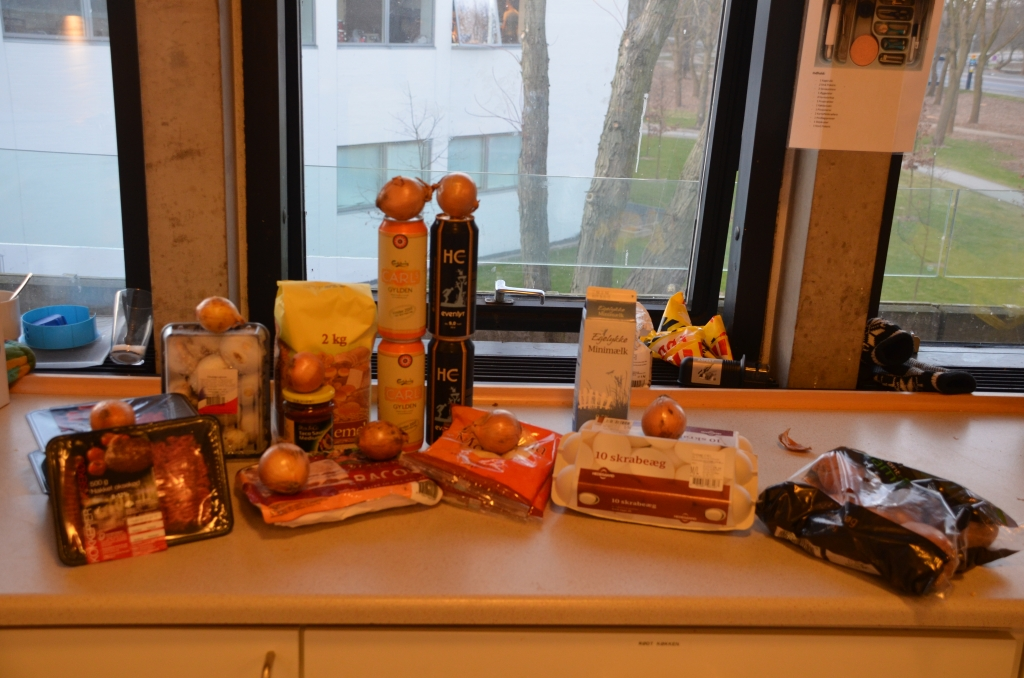
\includegraphics[width=0.8\columnwidth]{/KABSmad/1}
\caption{Madingredienserne}
\end{figure}

\begin{figure}[h!]
\centering
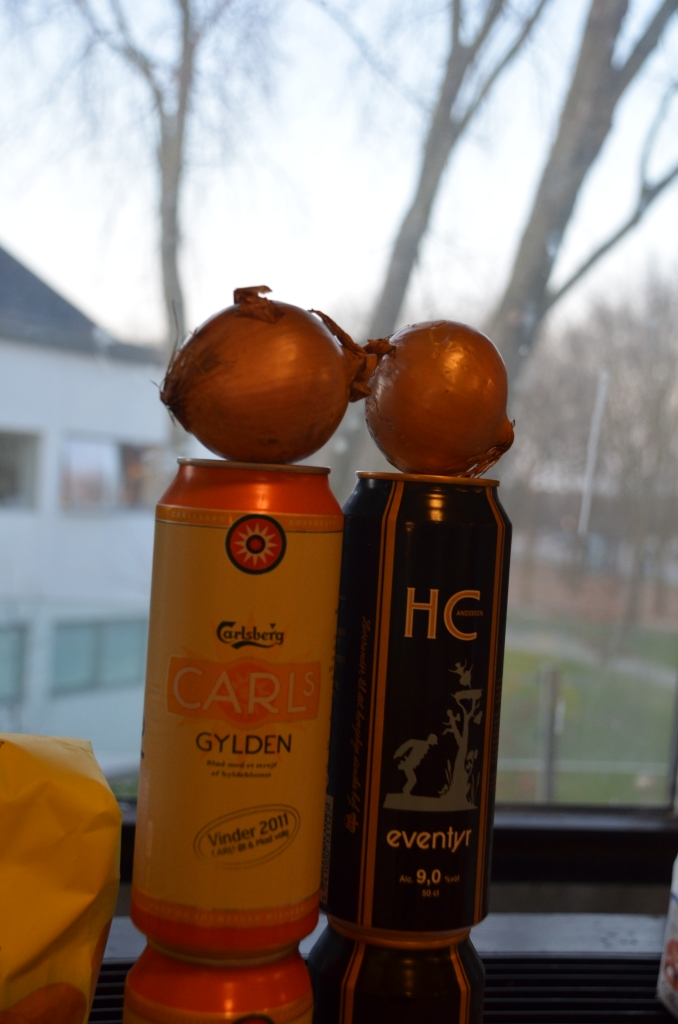
\includegraphics[width=0.5\columnwidth]{/KABSmad/2}
\caption{Den anerkendte eventyr som en hver morgen skal startes med på hyttetur, akkompagneret af en Carls Gylden }
\end{figure}

\begin{figure}[h!]
\centering
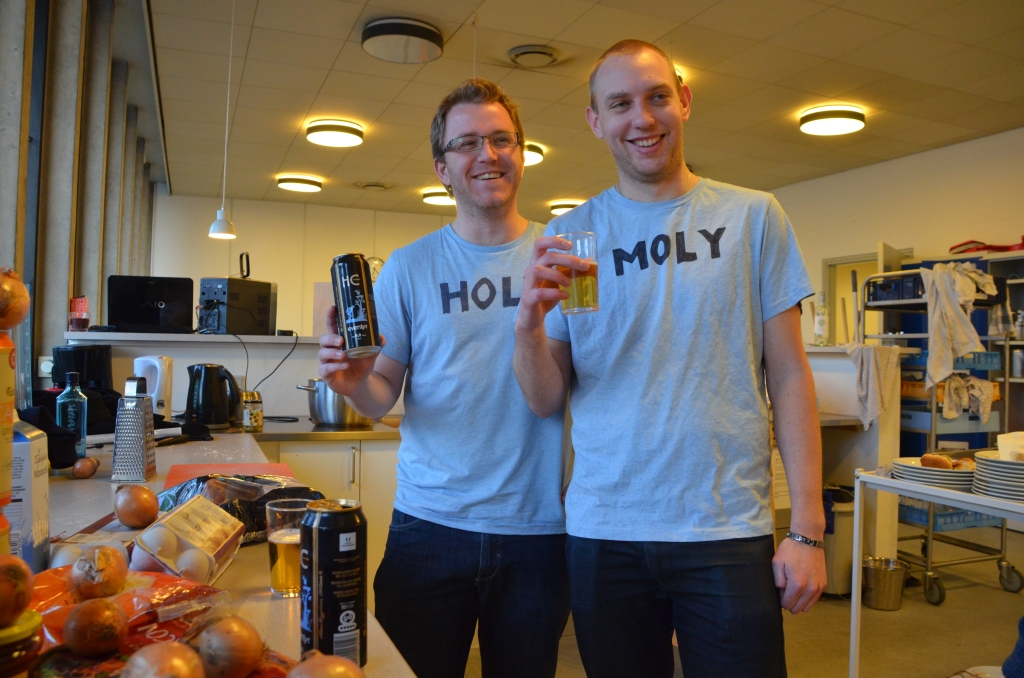
\includegraphics[width=0.6\columnwidth]{/KABSmad/3}
\caption{En skål er altid vigtig under madlavning. Bemærk \HM t-shirtsene }
\end{figure}

\begin{figure}[h!]
\centering
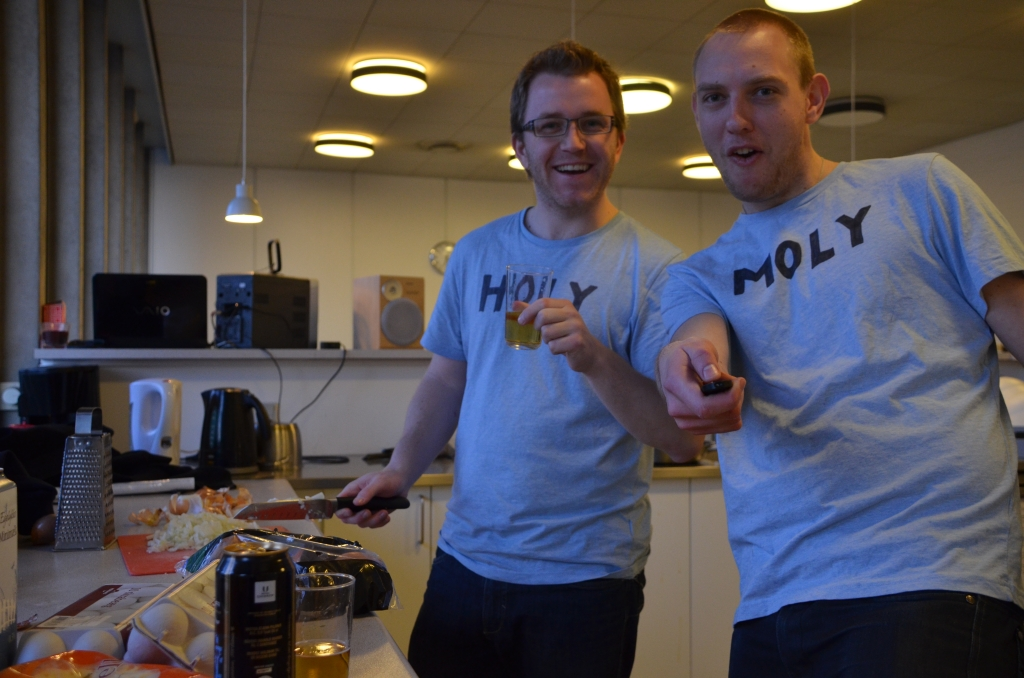
\includegraphics[width=0.6\columnwidth]{/KABSmad/4}
\caption{Ingen kommentar}
\end{figure}

\begin{figure}[h!]
\centering
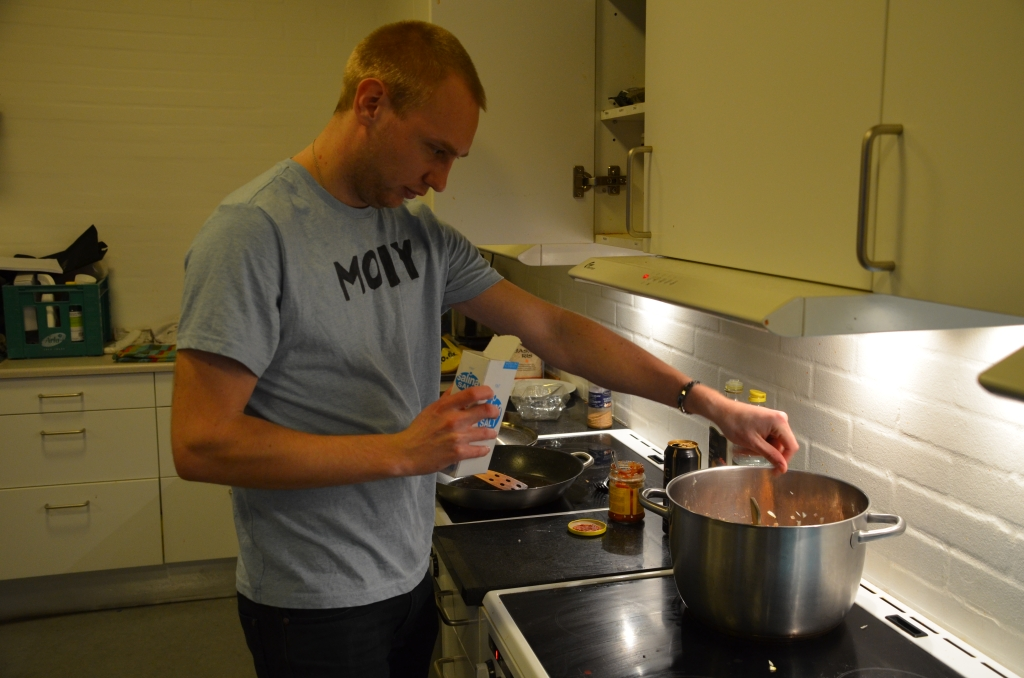
\includegraphics[width=0.6\columnwidth]{/KABSmad/5}
\caption{Altid vigtigt at have en saltefanden \cite{bib:url:Saltefanden} med}
\end{figure}

\begin{figure}[h!]
\centering
\subfigure[Et smil på læben mens dejen laves]{
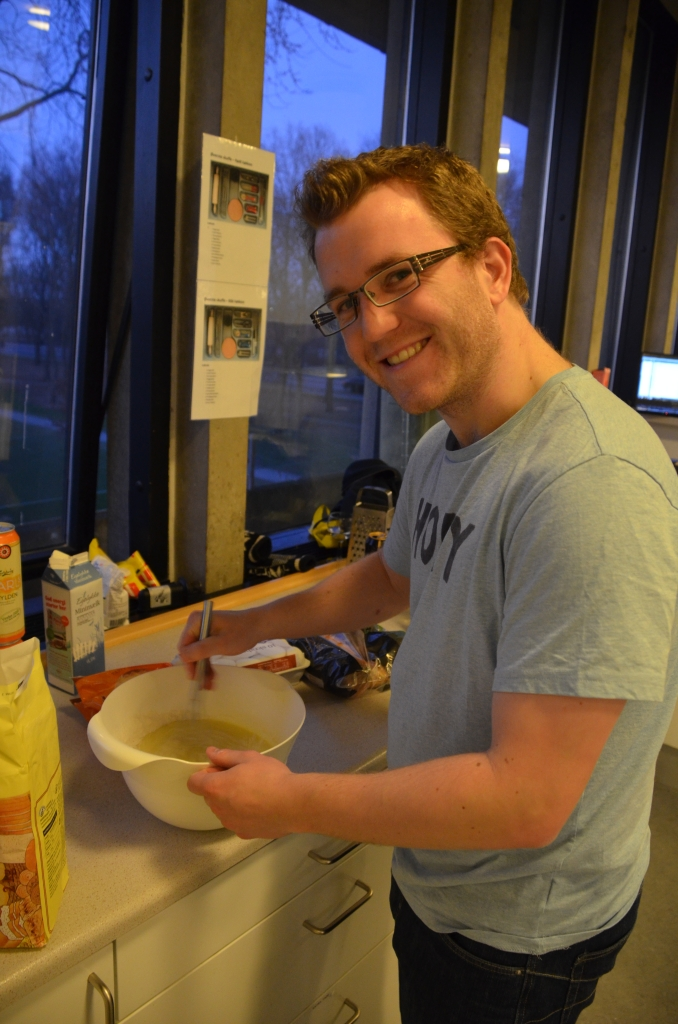
\includegraphics[width=0.45\columnwidth]{/KABSmad/6}
}
\subfigure[... og pandekagerne laves.]{
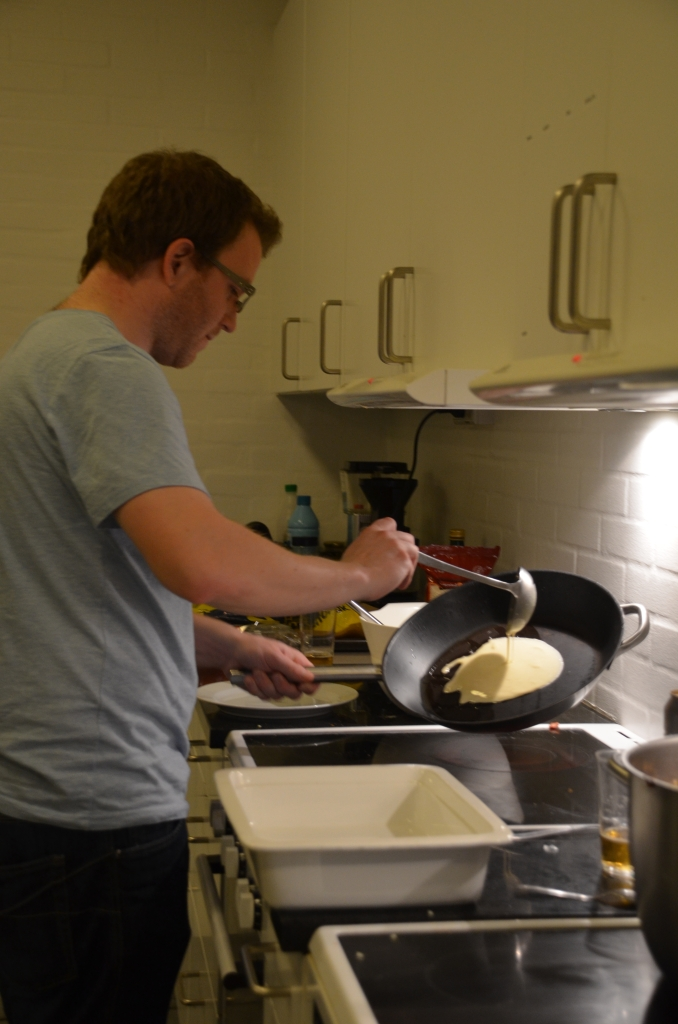
\includegraphics[width=0.45\columnwidth]{/KABSmad/7}
}
\caption{Pandekager laves}
\label{fig:app1}
\end{figure}

\begin{figure}[h!]
\centering
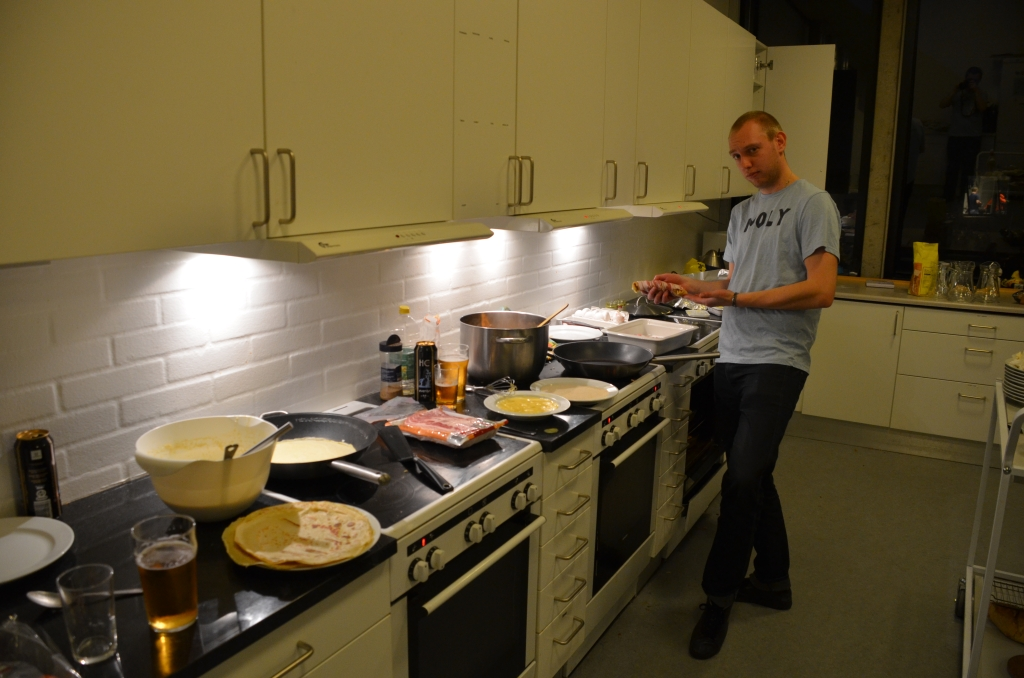
\includegraphics[width=0.8\columnwidth]{/KABSmad/8}
\caption{Et overblik over produktionslinjen. Produktet er blevet wrappet i bacon og er på vej ind i ovnen.}
\end{figure}

\begin{figure}[h!]
\centering
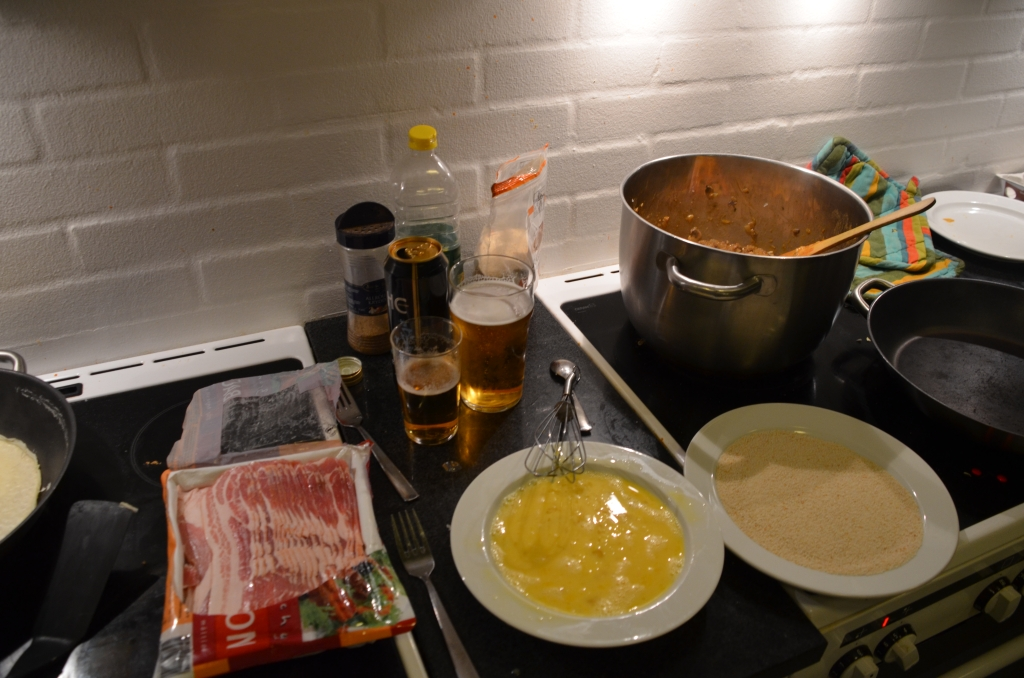
\includegraphics[width=0.8\columnwidth]{/KABSmad/9}
\caption{Close up overblik af panerings produktionslinjenm.}
\end{figure}


\begin{figure}[h!]
\centering
\subfigure[I henhold til figur \ref{fig:FoodBeer} skal man huske at drikke øl.]{
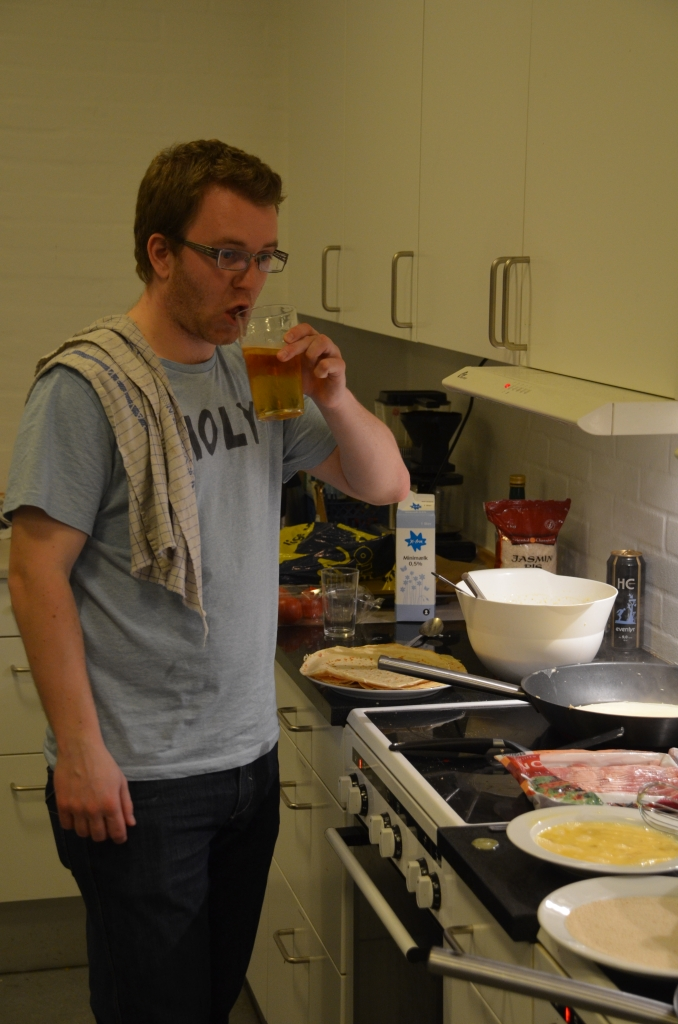
\includegraphics[width=0.45\columnwidth]{/KABSmad/10}
}
\subfigure[Som rigtig kok smager man selvfølgelig på maden for at opretholde den høje madkvalitet.]{
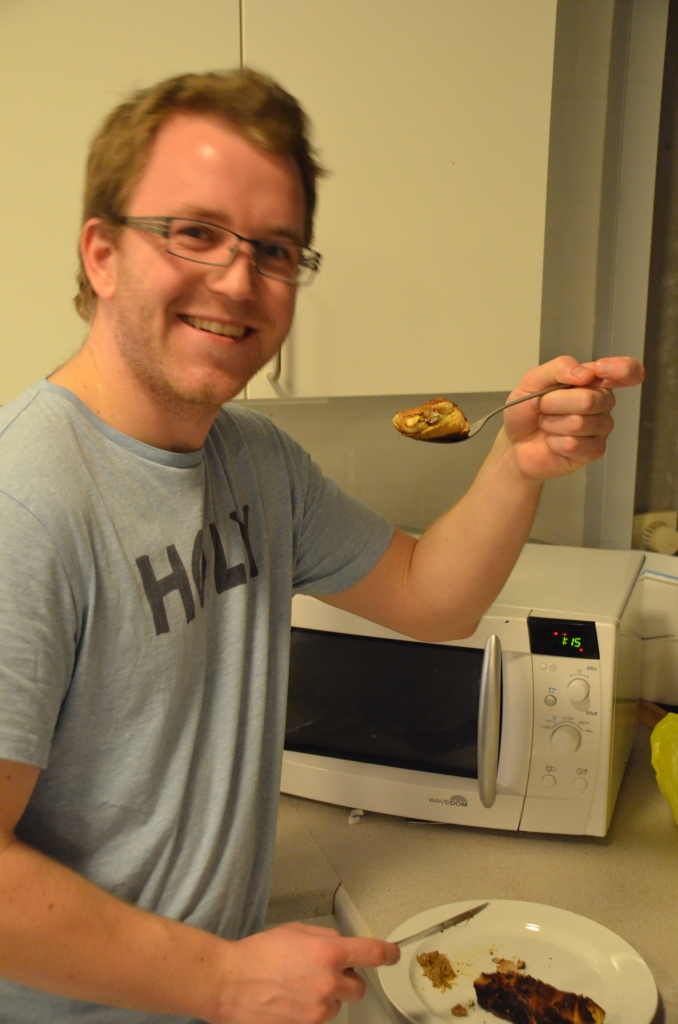
\includegraphics[width=0.45\columnwidth]{/KABSmad/11}
}
\caption{Ølsmagning og madsmagning.}
\label{fig:app2}
\end{figure}

\begin{figure}[h!]
\centering
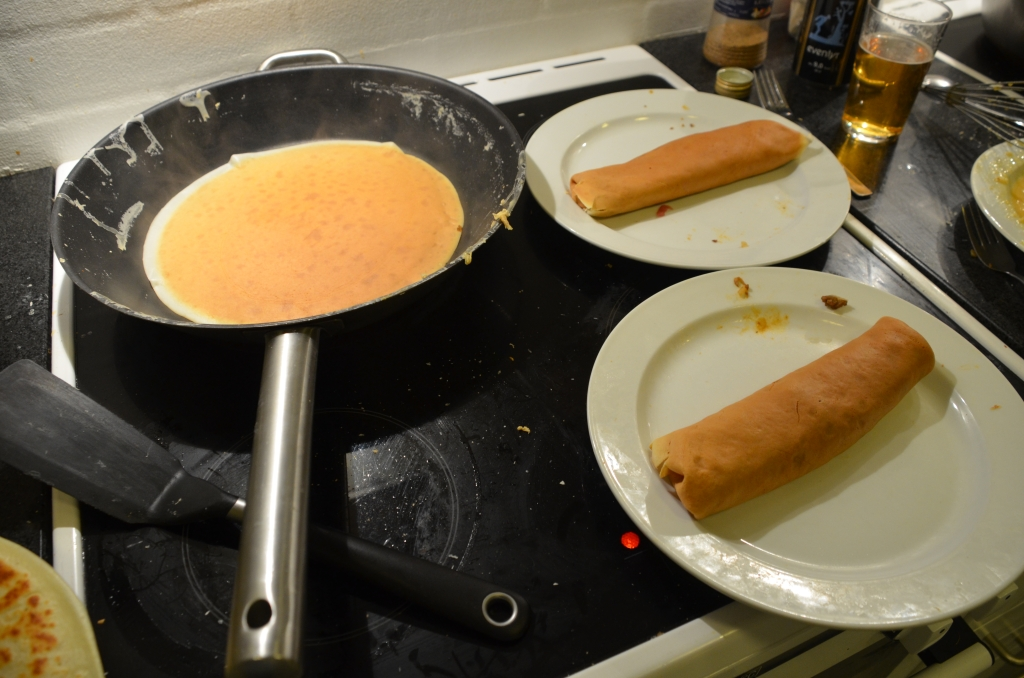
\includegraphics[width=0.6\columnwidth]{/KABSmad/14}
\caption{Pandekager klar til at blive wrapped.}
\end{figure}

\begin{figure}[h!]
\centering
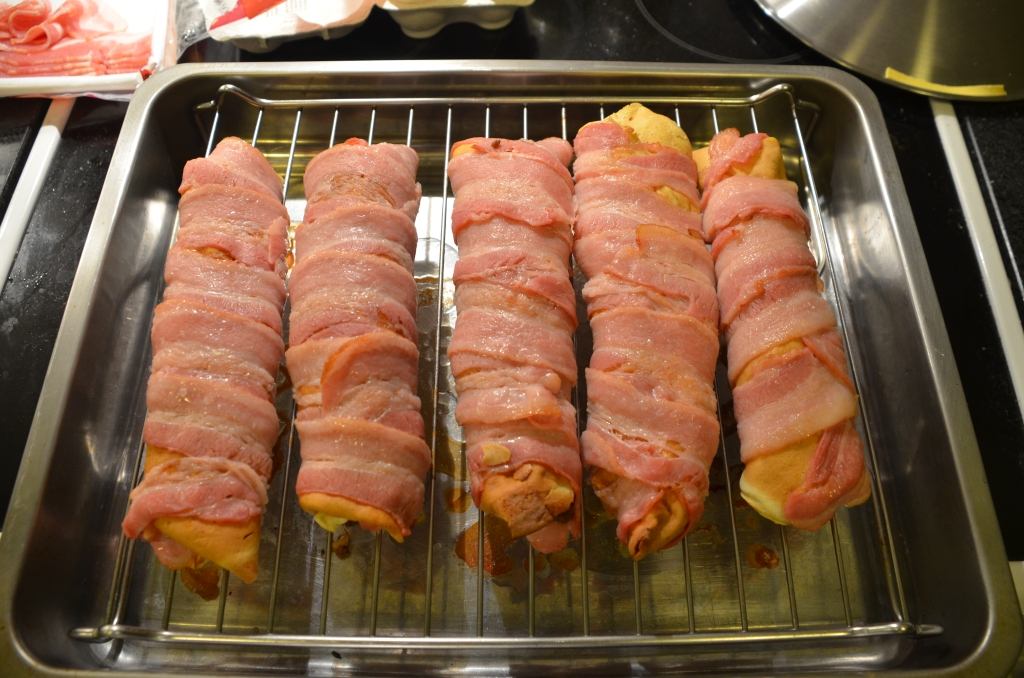
\includegraphics[width=0.6\columnwidth]{/KABSmad/13}
\caption{Pandekager wrapped i bacon klar til ovnen.}
\end{figure}

\begin{figure}[h!]
\centering
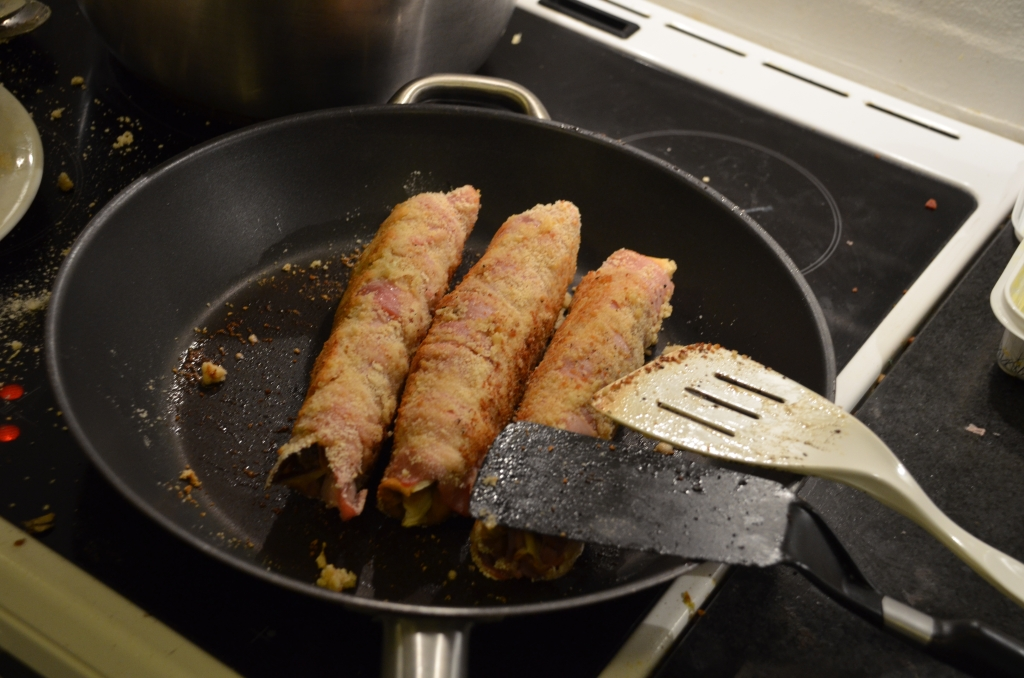
\includegraphics[width=0.6\columnwidth]{/KABSmad/15}
\caption{Pandekager under panering.}
\end{figure}

\begin{figure}[h!]
\centering
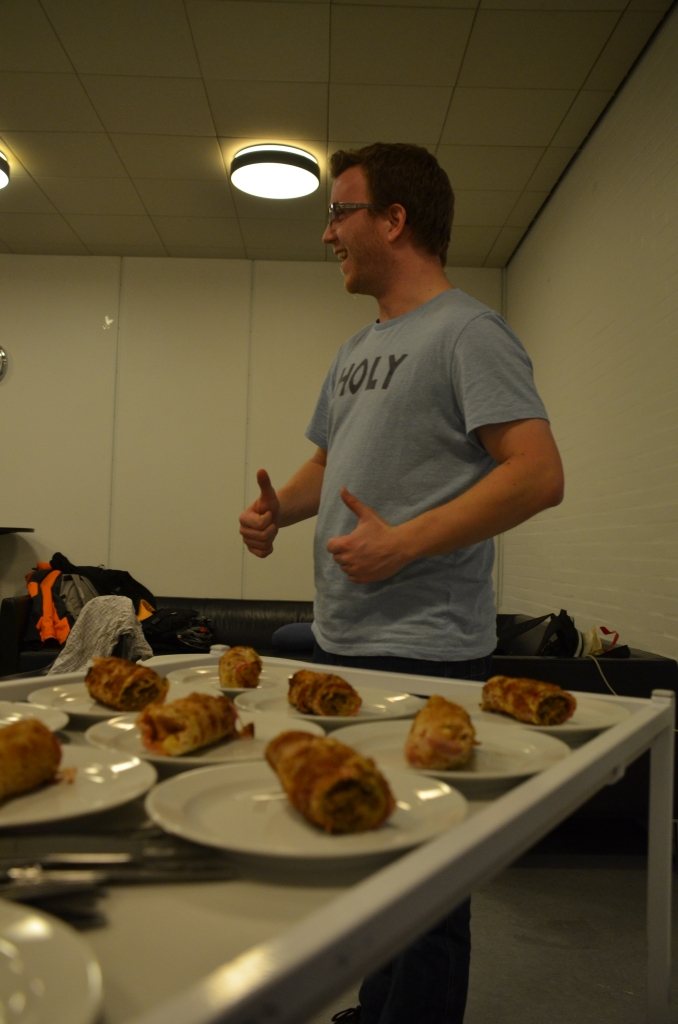
\includegraphics[width=0.5\columnwidth]{/KABSmad/16}
\caption{Færdig paneret pandekager klar til servering. Notér de to thumbs-up som signalerer høj madkvalitet.}
\end{figure}

\begin{figure}[h!]
\centering
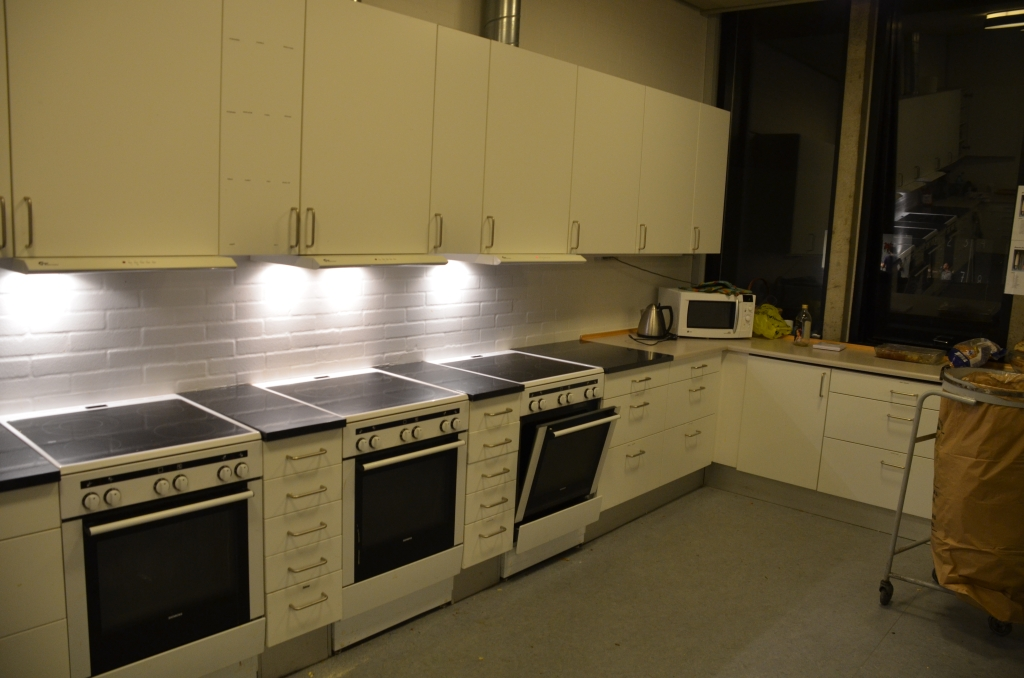
\includegraphics[width=0.8\columnwidth]{/KABSmad/17}
\caption{Køkkenet efter fuldendt madlavning. Renere end nogensinde set før.}
\end{figure}